\section{Apresentação}

\begin{frame}%{Capa}
    \titlepage
\end{frame}

\begin{frame}[c]{Apresentação}
    \begin{itemize}
        \item Professor Rodrigo de Farias Gomes
        \item Telefone (somente mensagens): (92) 9 9405-1724
        \item E-mail: shpnft@gmail.com
    \end{itemize}
\end{frame}

\begin{frame}{Ementa}
    \begin{itemize}
        \item Equilíbrio Estático (somente Química Industrial)
        \item Fluidos
        \item Oscilações
        \item Ondas em meio material
        \item Ondas sonoras
        \item Temperatura e calor
        \item Primeira lei da termodinâmica
        \item Teoria cinética dos gases
        \item Segunda lei da temodinâmica
        \item Ciclo de Carnot
    \end{itemize}
\end{frame}

\begin{frame}{Avaliação}
    \begin{itemize}
        \item A avaliação será na forma de 3 notas: \(N_1\), \(N_2\) e \(N_3\)
        \item A média dos exercícios escolares (\(MEE\)) será dada por
            \[
                MEE=\frac{N_1+N_2+N_3}{3}
            \]
        \item Se \(MEE \geq 8,0\), então a média final (\(MF\)) será igual à \(MEE\)
        \item Se \(MEE < 8,0\), então
            \[
                MF=\frac{2\times MEE+PF}{3}
            \]
            onde PF é a nota da \textbf{prova final}
        \item Se \(MF \geq 5,0\) e a frequência em sala for maior que 75\%, o aluno está aprovado
    \end{itemize}
\end{frame}

\begin{frame}[c]{Livro texto}
    \begin{center}
        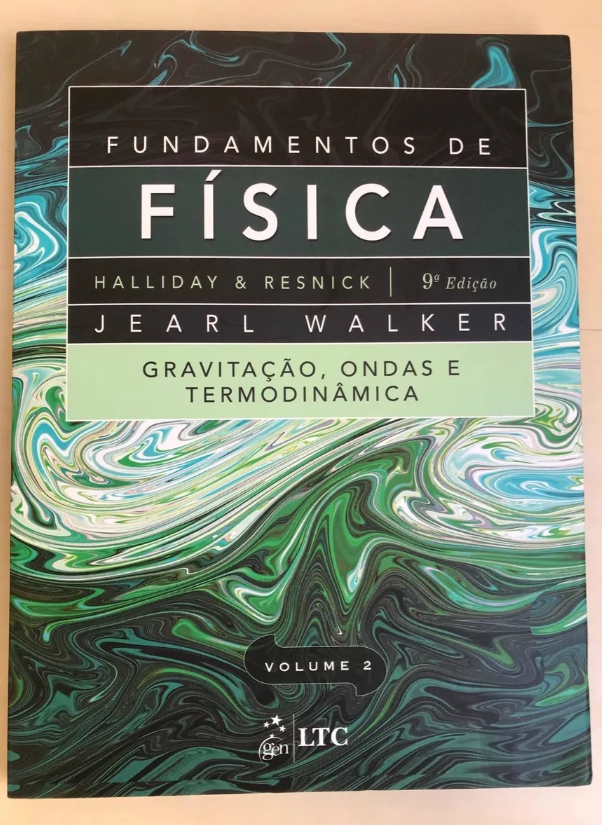
\includegraphics[width=0.33\textwidth]{images/halliday_9.png}
        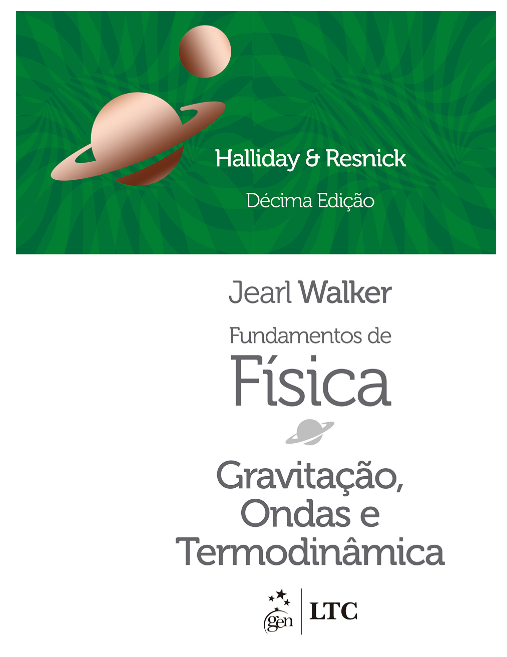
\includegraphics[width=0.33\textwidth]{images/halliday_10.png}
    \end{center}
\end{frame}

\section{Equilíbrio estático}

\begin{frame}{Força e torque}
    \begin{itemize}
        \item Forças causam variação no movimento \textbf{translacional}
        \item Torques causam variação no movimento \textbf{rotacional}
    \end{itemize}
    \begin{center}
        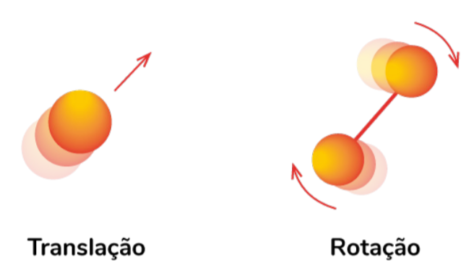
\includegraphics[width=6cm]{images/translação-rotação.png}
    \end{center}
    \pause
    Dessa forma, o que é necessário para que um corpo rígido esteja em \textbf{equilíbrio estático}?
\end{frame}

\begin{frame}{Equilíbrio estático}
    \begin{itemize}[<+->]
        \item A força externa resultante que atua sobre o corpo deve ser nula:
            \[
                \sum \vec{F}=\vec{0} \implies
                \begin{cases}
                    \sum F_x =0 \\ \sum F_y =0 \\ \textcolor{blue}{\sum F_z =0}
                \end{cases}
            \]

        \item O torque externo resultante deve ser nulo:
            \[
                \sum \vec{\tau}=\vec{0} \implies
                \begin{cases}
                    \textcolor{blue}{\sum \tau_x =0} \\
                    \textcolor{blue}{\sum \tau_y =0} \\
                    \sum \tau_z =0
                \end{cases}
            \]
    \end{itemize}
\end{frame}

\begin{frame}{Atividade}
    \begin{center}
        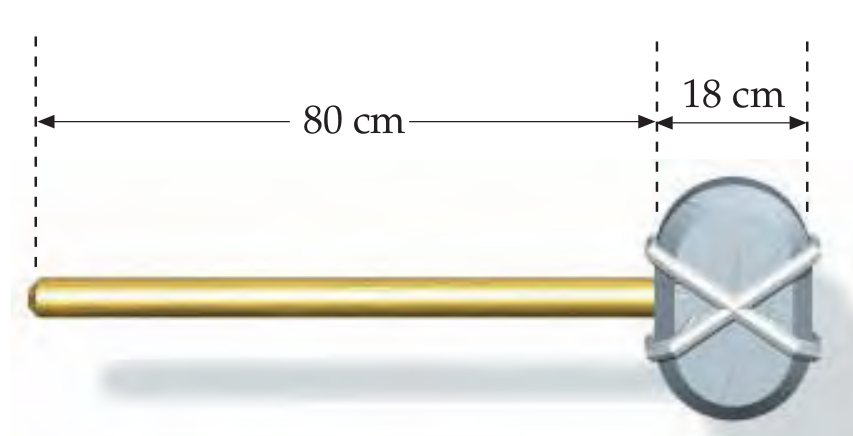
\includegraphics[width=0.5\textwidth]{images/thor}
    \end{center}
    Na figura acima, se a cabeça do martelo pesa \SI{8}{kg} e o cabo pesa \SI{2.5}{kg}, a que distância da extremidade
    esquerda do martelo devemos amarrar um fio para que ele fique na horizontal quando pendurado? Considere tanto
    a cabeça quanto o cabo do martelo \textbf{uniformes}

    \pause

    \begin{itemize}
        \item Data de entrega: 20/10
        \item Vale 1 ponto extra na \(N_1\) (nota máxima 10)
    \end{itemize}
\end{frame}

\begin{frame}{Centro de massa}
    \begin{itemize}
        \item O centro de massa de um sistema de partículas é o ponto que se move como se (1) toda a massa do sistema estivesse
            concentrada nesse ponto e (2) todas as forças externas estivessem aplicadas nesse ponto
        \item Se o sistema de partículas é \textit{discreto}, temos
            \[
                \vec{r}_{CM} = \frac{1}{M} \sum_{i=1}^{N} m_i \vec{r}_i
            \]
        \item Se o sistema de partículas é \textit{contínuo}, temos
            \[
                \vec{r}_{CM} = \frac{1}{M} \int \vec{r}\; dm
            \]
    \end{itemize}
\end{frame}

\begin{frame}[c]{Centro de gravidade}
    \begin{itemize}
        \item A força gravitacional \( \vec{F}_g\) age \textit{efetivamente} sobre um único ponto de um corpo, o chamado \textbf{centro de
        gravidade} (CG) do corpo
    \item Se \( \vec{g}\) é igual para todos os elementos de um corpo, o centro de gravidade (CG) do corpo coincide com o centro
        de massa (CM)

    \item O torque devido a \(\vec{F}_g\) pode ser calculado como se \(\vec{F_g}\) estivesse aplicada \textit{somente} no centro de gravidade
    \end{itemize}
\end{frame}

\begin{frame}{Exemplo 1}
    Uma esfera homogênea de massa \( m = \SI{0.85}{kg} \) e raio \(r = \SI{4.2}{cm}\) é mantida em repouso
    por uma corda, de massa desprezível, presa a uma parede sem atrito a uma distância \(L = \SI{8.0}{cm}\) acima do
    centro da esfera. Determine (a) a tração da corda e (b) a força que a parede exerce sobre a esfera.
    \begin{center}
        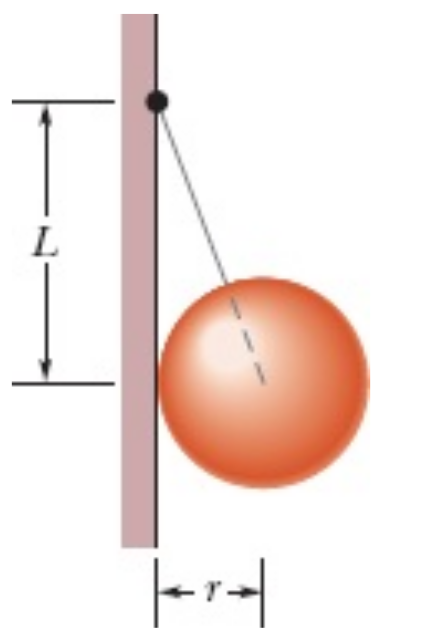
\includegraphics[width=0.2\textwidth]{images/bolapendurada}
    \end{center}
\end{frame}

\begin{frame}{Torque}
    \begin{itemize}
        \item Temos que
            \begin{align*}
                \vec{\tau} &= \vec{r} \times \vec{F} \\
                \tau &= r F \sen{\theta}
            \end{align*}
            onde \(\theta\) é o menor ângulo entre os vetores \(\vec{r}\) e \(\vec{F}\)
        \item Quando as forças e posições estão no \textbf{mesmo plano},
            a direção de \(\vec{\tau}\) é sempre perpendicular ao plano (''folha de papel''), mas o sentido depende da
            rotação que resultaria da ação do torque
            \begin{columns}
                \begin{column}{0.4\textwidth}
                    \begin{figure}
                        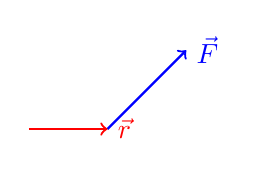
\begin{tikzpicture}[scale=0.5]
                            \draw [blue, thick, ->] (2,0) -- (4,2) node [right] { \(\vec{F}\) };
                            \draw [red, thick, ->] (0,0) -- (2,0) node [right] { \(\vec{r}\) };
                        \end{tikzpicture}
                        \caption{sentido positivo, saindo na folha de papel}
                    \end{figure}
                \end{column}

                \begin{column}{0.4\textwidth}
                    \begin{figure}
                        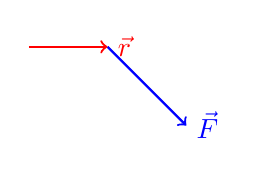
\begin{tikzpicture}[scale=0.5]
                            \draw [blue, thick, ->] (2,0) -- (4,-2) node [right] { \(\vec{F}\) };
                            \draw [red, thick, ->] (0,0) -- (2,0) node [right] { \(\vec{r}\) };
                        \end{tikzpicture}
                        \caption{sentido negativo, entrando da folha de papel}
                    \end{figure}
                \end{column}

            \end{columns}
    \end{itemize}
\end{frame}

\begin{frame}{''Os relógios são negativos...''}
    \centering
    \begin{tikzpicture}[scale=5]
        \draw[red,thick,->] (0,0,0) -- (1,0,0) node[below left]{$x$};
        \draw[blue, thick,->] (0,0,0) -- (0,1,0) node[below right]{$y$};
        \draw[black, thick,->] (0,0,0) -- (0,0,1) node[below right]{$z$};

        \only<1>{
        \draw[green!75!black, thick, ->] (0.5,0.5*tan{15}) arc (15:75:0.5/cos{15});
        \node [green!75!black, below] at (0.75,0.5) {rotação anti-horária};
        \draw [green!75!black,thick, ->] (0.3,0,0.25) -- (0.3,0,0.75) node [below] {sentido positivo};
    }
    \only<2>{
        \draw[magenta!75!black, thick, <-] (0.5,0.5*tan{15}) arc (15:75:0.5/cos{15});
        \node [magenta!75!black, below] at (0.75,0.5) {rotação horária};
        \draw [magenta!75!black,thick, ->] (0.3,0,0.75) node [below] {sentido negativo}-- (0.3,0,0.25);
    }
    \end{tikzpicture}
\end{frame}


\begin{frame}{Exemplo 2}

    \begin{minipage}{\textwidth}
        Romeu apoia uma escada uniforme de \SI{10}{m} em um muro liso (sem atrito).
        A massa da escada é \SI{22}{kg} e sua base, no chão, está a \SI{2.8}{m} do muro.
        Quando Romeu, cuja massa é \SI{70}{kg}, completa \SI{90}{\%} do percurso de subida, a escada começa a escorregar.
        Qual é o coeficiente de atrito estático entre o chão e a escada?
    \end{minipage}

    \begin{center}
        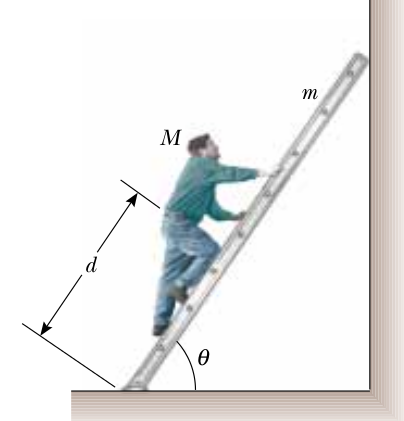
\includegraphics[width=0.3\textwidth]{images/romeu}
    \end{center}

\end{frame}

\begin{frame}{Exemplo 3}
    \begin{minipage}{\textwidth}
        Uma das extremidades de uma barra uniforme de \SI{4.00}{m} de comprimento e peso $F_g$ é sustentada por um cabo a um
        ângulo $\theta=\SI{37}{\degree}$ com a barra. A outra extremidade está apoiada na parede no ponto $A$, onde é segurada pelo atrito.
        O coeficiente de atrito estático entre a parede e a barra é $\mu_e=\num{0.500}$.
        Determine a distância mínima $x$ a partir do ponto $A$ na qual um corpo adicional com o mesmo peso da barra pode ser pendurado sem
        fazer com que a barra escorregue.
    \end{minipage}

    \begin{center}
        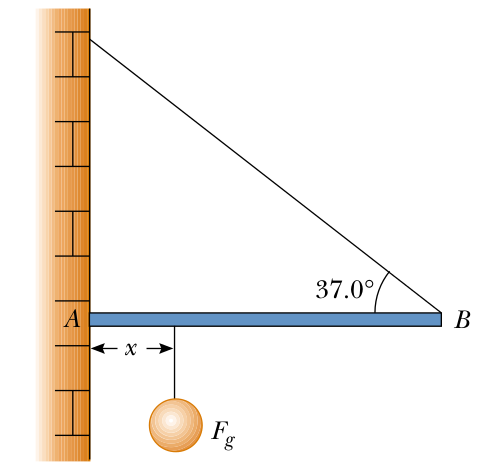
\includegraphics[width=0.25\textwidth]{images/pendurado}
    \end{center}
\end{frame}

% \begin{frame}{Exemplo 4}
%     \begin{minipage}{\textwidth}
%         Um alpinista de \SI{55}{kg} está subindo uma parede usando uma fissura na pedra, com as mãos puxando um
%         lado da fissura e os pés pressionando o lado oposto. A fissura tem uma largura w = \SI{0.20}{m},
%         e o centro de massa do alpinista está a uma distância horizontal d = \SI{0.40}{m} da fissura.
%         O coeficiente de atrito estático entre as mãos e a rocha é \(\mu_1 = \num{0.40}\)
%         e entre as botas e a pedra é \(\mu_2 = \num{1.2}\). (a) Qual é a menor força horizontal das
%         mãos e dos pés que mantém o alpinista estável? (b) Para a força horizontal do item (a),
%         qual deve ser a distância vertical h entre as mãos e os pés? Se o alpinista encontra uma pedra
%         molhada, para a qual os valores de \(\mu_1\) e \(\mu_2\) são menores, (c) o que acontece com a
%         resposta do item (a) e (d) o que acontece com a resposta do item (b)?
%     \end{minipage}
% \end{frame}

% \begin{frame}{}
%     \begin{center}
%         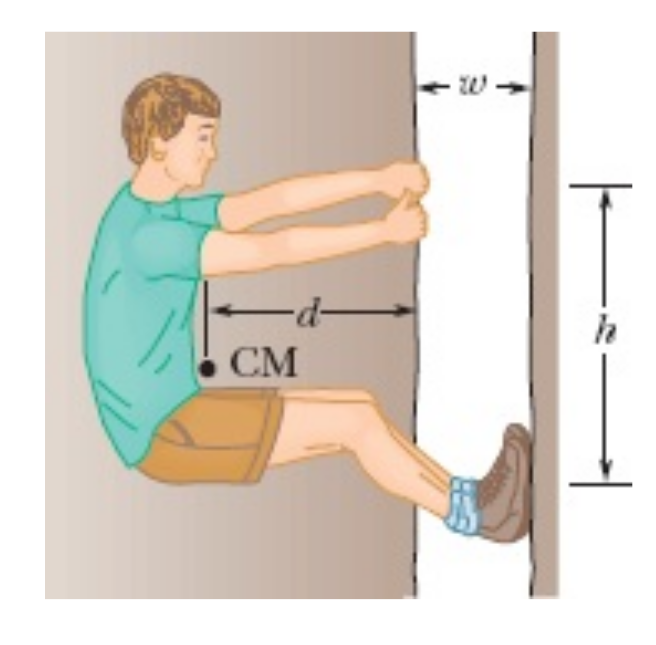
\includegraphics[width=0.5\textwidth]{images/Captura de tela de 2022-11-02 18-04-44.png}
%     \end{center}
% \end{frame}

\begin{frame}{Exemplo 4}
    \begin{minipage}{\textwidth}
        Um caixote, na forma de um cubo com \SI{1,2}{m} de lado, contém uma peça de máquina; o centro de
        massa do caixote e do conteúdo está localizado \SI{0,30}{m} acima do centro geométrico do caixote. O caixote
        repousa em uma rampa que faz um ângulo \(\theta\) com a horizontal. Quando \(\theta\) aumenta a partir de zero, um
        valor de ângulo é atingido para o qual o caixote tomba ou desliza pela rampa. Se o coeficiente de atrito
        estático \(\mu_s\) entre a rampa e o caixote é 0,60, (a) a rampa tomba ou desliza? (b) Para que ângulo \(\theta\) isso
        acontece? Se \(\mu_s\) = 0,70, (c) o caixote tomba ou desliza? (d) Para que ângulo \(\theta\) isso acontece? (Sugestão:
        Qual é o ponto de aplicação da força normal quando o caixote está prestes a tombar?)
    \end{minipage}
\end{frame}

\begin{frame}{Antes tarde do que nunca...}
    \begin{itemize}
        \item Como vimos, no caso em que forças e posições estão no mesmo plano \textit{xy}, o torque
            está ao longo do eixo \textit{z} e o sentido depende se a rotação que seria provocada é
            no sentido horário (negativo) ou anti-horário (positivo)
        \item Além disso, temos que o módulo do torque é dado por \(\tau = r F \sen{\theta}\)
        \item O detalhe que foi \textit{perdido} é que \textbf{podemos} decompor os vetores \(\vec{r}\) e \(\vec{F}\)
            em suas componentes \textit{x} e \textit{y} e, com isso, \textit{fugir} do cálculo/descoberta do
            ângulo \(\theta\)
        \item Isso é possível porque \(\vec{\tau} = \vec{r} \times \vec{F}\) é uma operação
            \textit{distributiva}\footnote{Mas tome cuidado: ela não é comutativa!}
        \item Assim
            \[
                \begin{cases}
                    \vec{r}=\vec{r_x}+\vec{r_y}\\
                    \vec{F}=\vec{F_x}+\vec{F_y}
                \end{cases}
                \implies
                \tau = r_x  F_y - r_y  F_x
            \]
            onde \(r_x\), \(r_y\), \(F_x\) e \(F_y\) são componentes, ou seja, \textbf{podem ser positivas ou negativas}

    \end{itemize}
\end{frame}

\begin{frame}{Torque do exemplo 4}
    \begin{columns}
        \begin{column}{0.45\textwidth}
            \begin{center}
                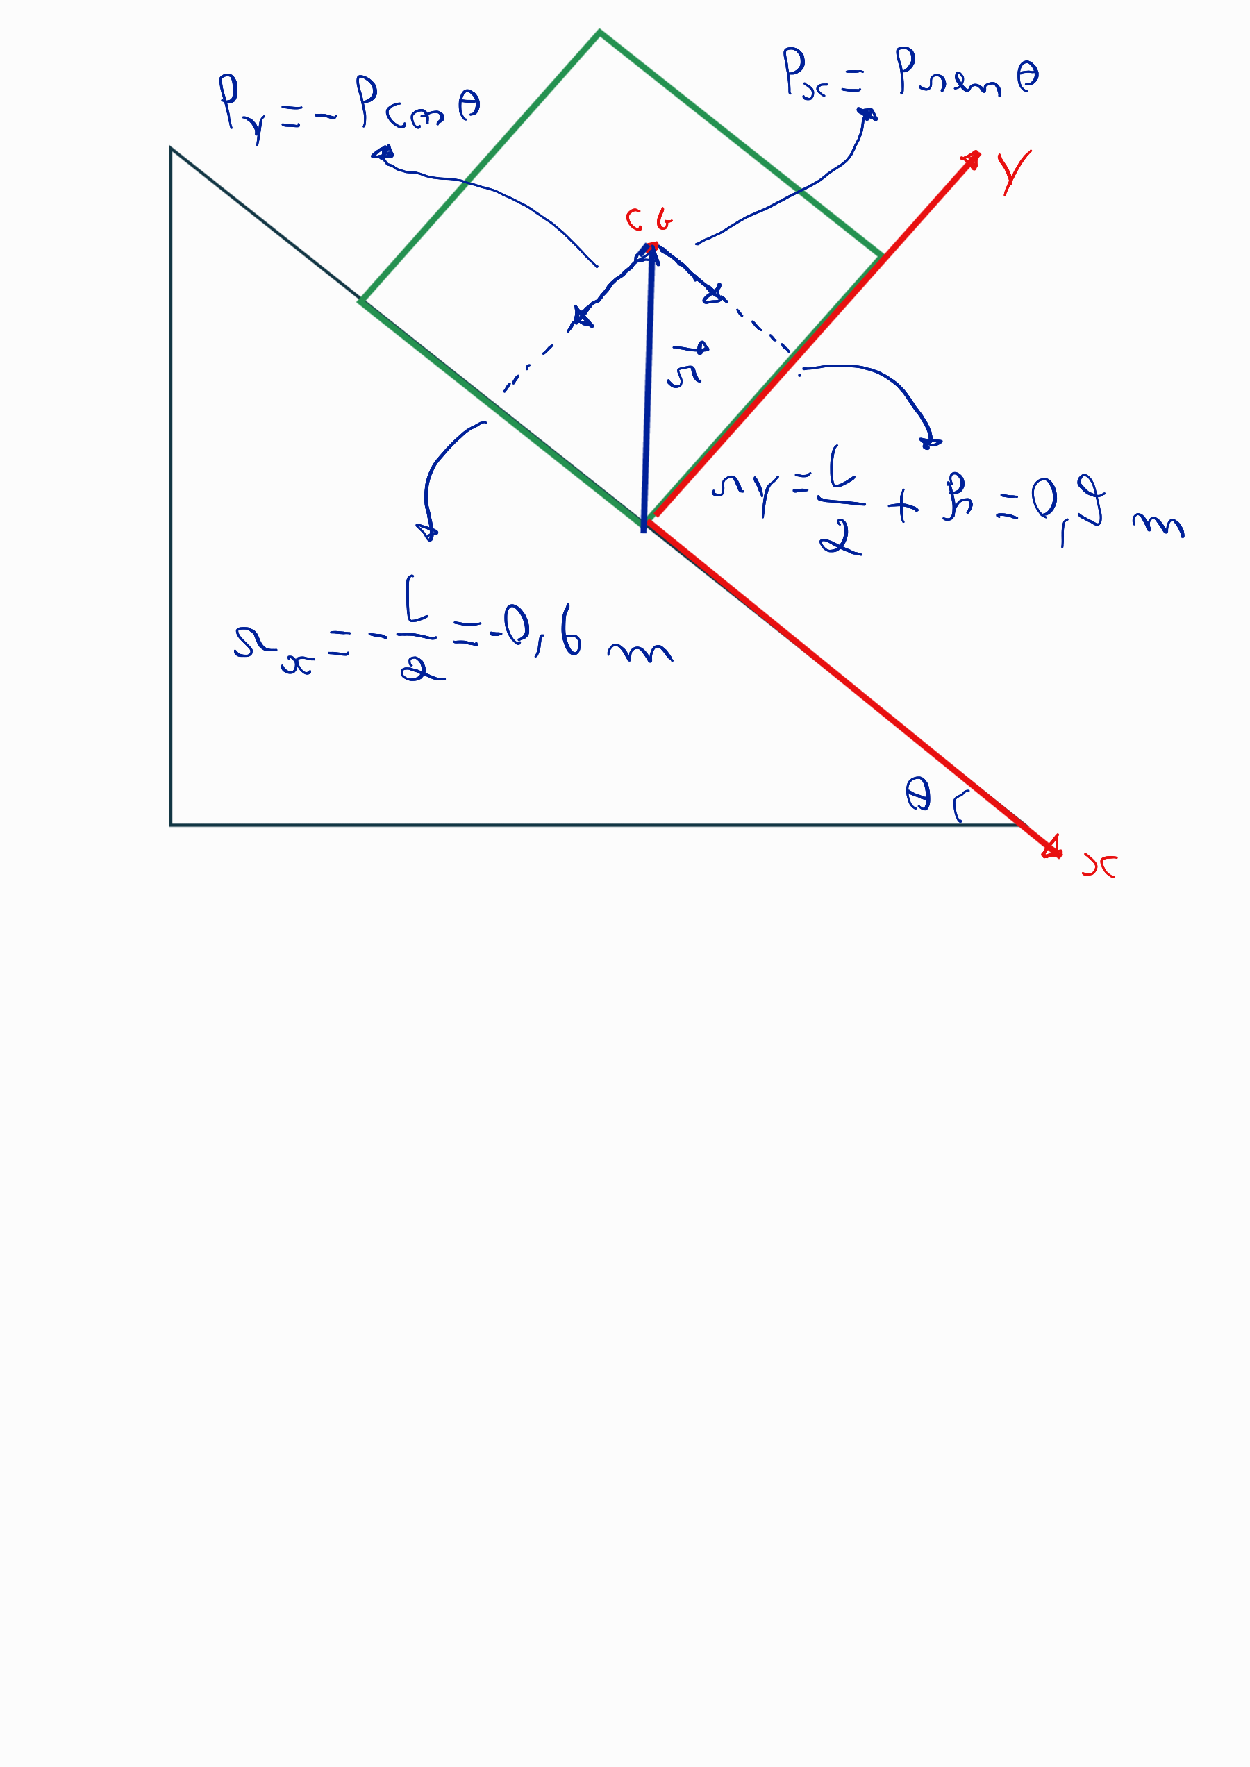
\includegraphics[width=\textwidth, trim={0 280pt 0 0}, clip]{images/torque-x.pdf}
            \end{center}
        \end{column}

        \begin{column}{0.5\textwidth}
            \begin{align*}
                \tau &= r_x  P_y - r_y  P_x \\
                     &= \left(- \frac{L}{2}\right) \left( -P\cos{\theta}\right)-\left(\frac{L}{2}+h\right)\left(P\sen{\theta}\right) \\
                     &= 0
            \end{align*}

            ou seja,
            \[
                \tan{\theta} = \frac{\frac{L}{2}}{\frac{L}{2}+h}
                = \frac{\SI{0,6}{m}}{\SI{0,9}{m}}
                \implies \theta = \SI{33,7}{\degree}
            \]
            de acordo com o que foi obtido na última aula
        \end{column}
    \end{columns}

\end{frame}


\begin{frame}{Atividade}

    \begin{itemize}
        \item Essa atividade vale 25\% da \(N_1\)
        \item É um \textbf{estudo dirigido}, isto é, os alunos podem tirar dúvidas com o professor
        \item Grupo de até 2 alunos
        \item Resolva os problemas 11, 17, 31 e 37 do capítulo 12 do livro texto
        \item Data de entrega: 24/11/2022
    \end{itemize}

\end{frame}

\section{Fluidos}

\begin{frame}{Fluidos}
    \begin{itemize}
        \item Um fluido é uma substância que pode escoar, assumindo a forma do recipiente em que é colocado
        \item Quando discutimos corpos rígidos, as grandezas físicas que usamos são \textbf{massa} e \textbf{força}
            \begin{center}
                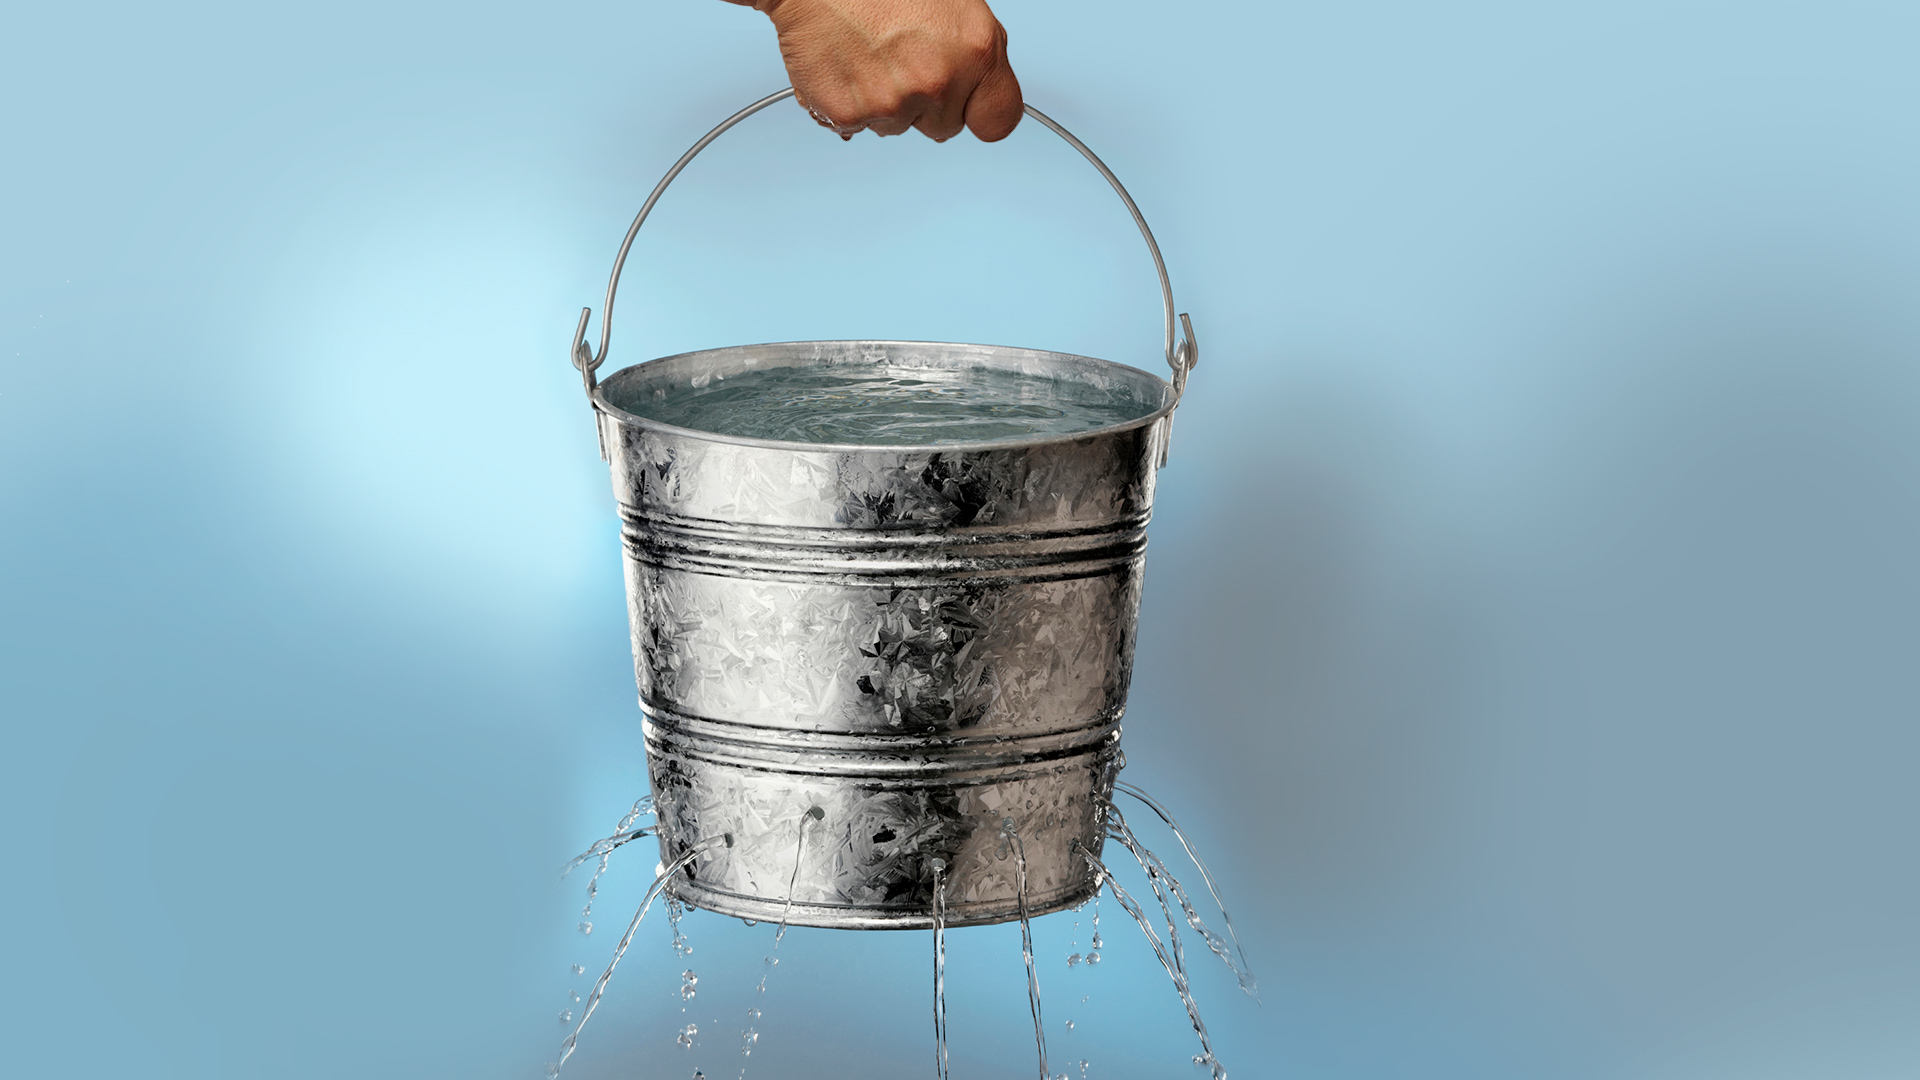
\includegraphics[width=0.6\textwidth]{images/balde_furado.jpg}
            \end{center}
        \item No caso de fluidos, é mais útil falar em \textbf{massa específica} e \textbf{pressão}
    \end{itemize}
\end{frame}

\begin{frame}{Massa específica}
    \begin{itemize}
        \item A massa específica média de um corpo é dada por:
            \[
                \bar{\rho} = \frac{\Delta  m}{\Delta V}
            \]

        \item A massa específica de um ponto qualquer de um corpo é:
            \[
                \rho = \frac{dm}{dV}
            \]
        \item Para um corpo uniforme $\rho = \bar{\rho}$

        \item A unidade SI para a massa específica é o $\si{kg/m^3}$
    \end{itemize}

\end{frame}

\begin{frame}{Problema 14-1}
    \begin{minipage}{\textwidth}
        Um peixe se mantém na mesma profundidade na água doce ajustando a quantidade
        de ar em ossos porosos ou em bolsas de ar para tornar sua massa específica média
        igual à da água. Suponha que, com as bolsas de ar vazias, um peixe tem uma massa
        específica de \(\SI{1,08}{g/cm^3}\). Para que fração de seu novo volume o peixe deve inflar
        as bolsas de ar para tornar sua massa específica igual à da água?
    \end{minipage}

    \vspace{1cm}
    \textit{Dados:}
    \begin{itemize}
        \item Massa específica da água: \(\SI{1,00}{g/cm^3}\)
    \end{itemize}
\end{frame}

\begin{frame}{Pressão}

    \begin{itemize}
        \item A pressão $P$ sobre uma superfície é força por unidade de área:
            \[
                P=\frac{F}{A}
            \]
            onde $F$ é o módulo da força \textbf{normal à superfície} e $A$ é a área da superfície
        \item A pressão é uma grandeza \textbf{escalar} de onde podemos obter uma grandeza \textbf{vetorial} (força)

        \item Se a pressão \textbf{varia} sobre uma área, a força infinitesimal
            $dF$ sobre um elemento de superfície infinitesimal de área $dA$ é:
            \[
                dF=P dA
            \]
        \item A unidade SI para a pressão é o pascal: $\SI{1}{Pa} = \SI{1}{N/m^2}$
    \end{itemize}
\end{frame}

\begin{frame}{Outras unidades de pressão}
    Além do pascal, também são comumente usadas:
    \begin{fleqn}
        \begin{gather*}
            \SI{1}{atm} = \SI{101.325}{kPa} \\
            \SI{1}{bar} = \SI{100}{kPa} \\
            \SI{1}{psi} = \SI{1}{lbf/in^2} = \frac{\SI{4.4482}{N}}{(\SI{0.0254}{m})^2} =
            \SI{6894.7548}{Pa} \\
            \SI{1}{atm} = \SI{14.7}{psi}
        \end{gather*}
    \end{fleqn}
\end{frame}

\begin{frame}{}
    \begin{center}
        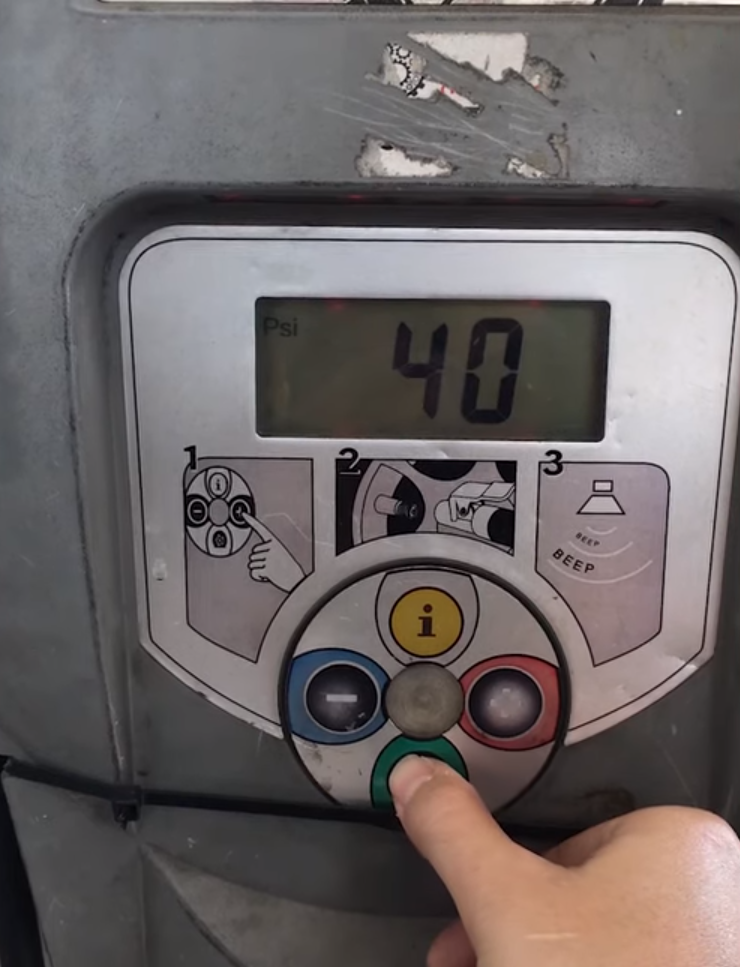
\includegraphics[height=8cm]{images/psi.png}
    \end{center}
\end{frame}

\begin{frame}{Pressão em Fluidos}
    \begin{itemize}
        \item A pressão em um fluido aumenta com a profundidade
        \item A pressão em um fluido \textbf{incompressível} aumenta \textbf{linearmente} com a profundidade
            \[
                P=P_0 + \rho g h
            \]
        \item \textbf{Princípio de Pascal}: Variações de pressão aplicadas em
            um fluido \textbf{incompressível} confinado são transmitidas, sem
            redução, a todos os pontos do fluido e às paredes do recipiente
            \[
                \Delta P_1 = \Delta P_2 = \ldots = \Delta P_n
            \]
    \end{itemize}
\end{frame}

\begin{frame}{Problema 14-4}
    \begin{minipage}{\textwidth}
        Três líquidos imiscíveis são despejados em um recipiente cilíndrico. Os volumes e
        massas específicas são:
        \begin{enumerate}
            \item \SI{0,50}{L} e \(\SI{2,6}{g/cm^3}\)
            \item \SI{0,25}{L} e \(\SI{1,0}{g/cm^3}\)
            \item \SI{0,40}{L} e \(\SI{0,80}{g/cm^3}\)
        \end{enumerate}
        Qual é a força total exercida pelos líquidos sobre o fundo do recipiente? Ignore
        a contribuição da atmosfera.
    \end{minipage}

    \vspace{1cm}
    \textit{Dados:} \SI{1}{L} =  \(\SI{1000}{cm^3}\)
\end{frame}

\begin{frame}{Exemplo 13-3 do Tipler}
    \begin{minipage}{\textwidth}
        O pistão grande de um elevador hidráulico tem um raio de \SI{20}{cm}.
        Qual é a força que deve ser aplicada sobre o pistão pequeno, de
        \SI{2.0}{cm} de raio, para levantar um carro de \SI{1500}{kg} de massa?
    \end{minipage}
    \begin{center}
        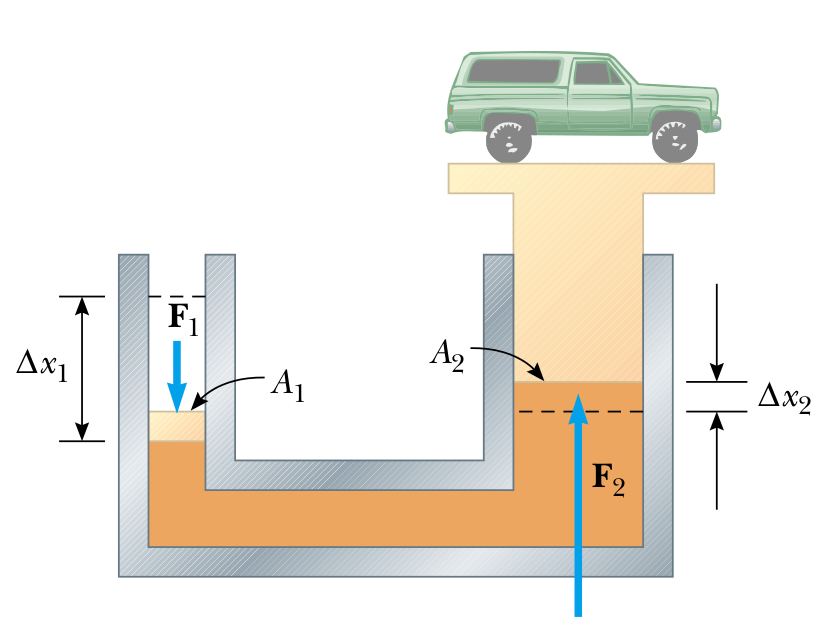
\includegraphics[width=0.45\textwidth]{images/pistao}
    \end{center}
\end{frame}

\begin{frame}{Seção 14.3 do Serway}
    \begin{minipage}{\textwidth}
        A figura seguinte mostra um barômetro de mercúrio, que é usado para
        medir a pressão atmosférica. Se a massa específica do mercúrio é
        $\SI{13.6e3}{kg/m^3}$, qual a altura da coluna de mercúrio se a pressão
        $P_0 = \SI{101.3}{kPa}$?
    \end{minipage}
    \begin{center}
        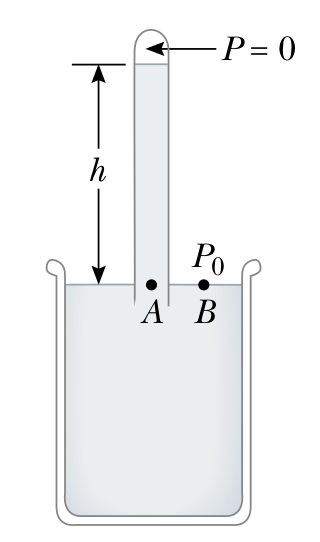
\includegraphics[width=0.2\textwidth]{images/barometro}
    \end{center}
\end{frame}

\begin{frame}{Problema 14-10}
    \begin{minipage}{\textwidth}
        O tubo de plástico da figura abaixo tem uma seção reta de \(\SI{5,00}{cm^2}\).
        Introduz-se água no tubo até o lado mais curto (de comprimento \(d= \SI{0,800}{m}\) fique
        cheio. Em seguida, o lado menor é fechado e mais água é despejada no lado maior. Se a tampa do lado menor
        é arrancada quando a força a que está submetida excede \SI{9,80}{N}, que altura da coluna de água do lado
        maior deixa a tampa na iminência de ser arrancada?
    \end{minipage}

    \vspace{1cm}\centering
    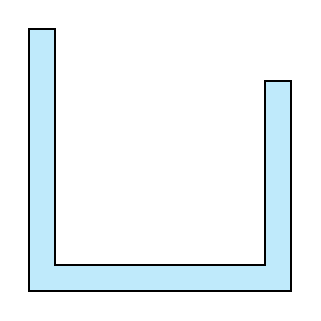
\begin{tikzpicture}[scale=1/3]
        \draw [thick, fill=cyan!25] (0,10) -- (0,0) -- (10,0) -- (10,8) --  (9,8) -- (9,1) -- (1,1) -- (1,10) -- cycle;
    \end{tikzpicture}
\end{frame}

\begin{frame}{Problema 14-81}
    \begin{minipage}{\textwidth}
        Seja um tubo em forma de U modificado: o lado direito é mais curto que o lado
        esquerdo. A extremidade do lado direito está \(d=\SI{10,0}{cm}\) acima da bancada do laboratório.
        O raio do tubo é \SI{1,50}{cm}. Despeja-se água, lentamente, no lado esquerdo até que comece a
        transbordar do lado direito. Em seguida, um líquido, de massa específica \(\SI{0,80}{g/cm^3}\), é despejado
        lentamente no lado esquerdo até que a altura do líquido nesse lado seja de \SI{8,0}{cm} (o líquido não
        se mistura com a água). Que quantidade de água transborda do lado direito?
    \end{minipage}
\end{frame}

\begin{frame}{Exemplo 13-2 do Tipler}
    \begin{minipage}{\textwidth}
        Uma represa retangular de \SI{30}{m} de largura suporta uma quantidade
        de água de \SI{25}{m} de profundidade. Determine a força horizontal
        total sobre a represa, exercida pela água e pela pressão atmosférica
        $P_0 = \SI{101.3}{kPa}$.
    \end{minipage}
    \begin{center}
        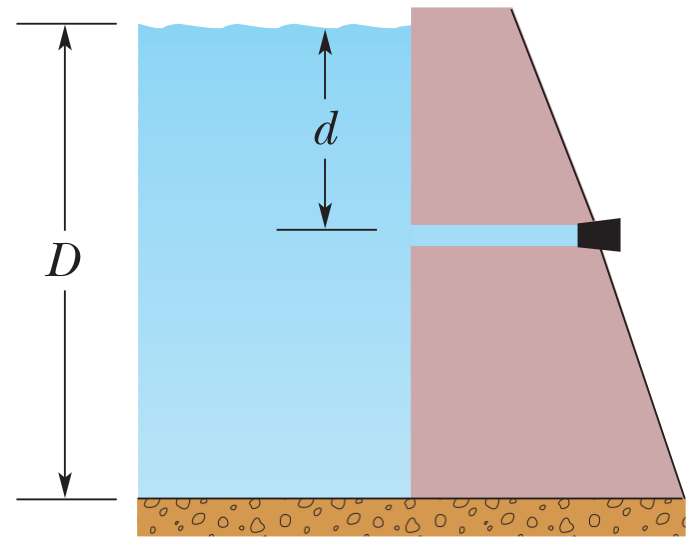
\includegraphics[width=0.45\textwidth]{images/represa}
    \end{center}
\end{frame}

\begin{frame}{Princípio de Arquimedes}
    Um corpo total ou parcialmente mergulhado em um fluido sofre uma \textbf{força
    de empuxo} vertical de baixo para cima igual ao peso do fluido por ele
    deslocado:
    \[E=\rho g V_{sub}\]

    \begin{center}
        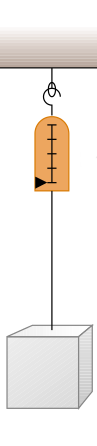
\includegraphics[height=0.4\textheight]{images/empuxo1}
        \hspace*{1cm}
        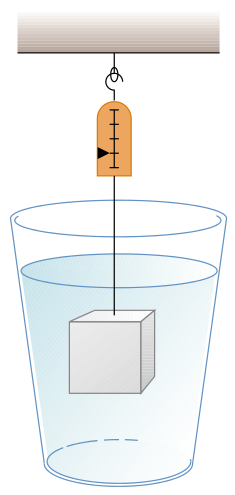
\includegraphics[height=0.4\textheight]{images/empuxo2}
    \end{center}

    O peso aparente $F_{ap}$ de um corpo imerso em um fluido é a diferença entre os
    módulos do seu peso $F_{g}$ e do empuxo $E$: \[F_{ap}=F_{g}-E\]
\end{frame}

\begin{frame}{Exemplo 1}
Diz a lenda que pediram a Arquimedes para determinar se uma coroa feita para o
rei consistia de ouro puro. Ele resolveu este problema pesando a coroa,
primeiro, no ar, e depois na água. Suponha que a balança tenha marcado
\SI{7.84}{N} quando a coroa estava no ar e \SI{6.84}{N} quando na água. Qual a
conclusão de Arquimedes, sabendo que a massa específica do ouro é
$\SI{19.3}{g/cm^3}?$
\end{frame}

\begin{frame}{Exemplo 2}
Um iceberg flutuando na água do mar é extremamente perigoso porque a maior
parte do gelo está abaixo da superfície. Que fração do volume de um iceberg
está abaixo do nível da água?

Dados:
\begin{itemize}
\item massa específica da água do mar: $\SI{1030}{kg/m^3}$
\item massa específica do gelo: $\SI{917}{kg/m^3}$
\end{itemize}

\end{frame}

\begin{frame}{Exemplo 3}
A porcentagem de gordura de seu corpo pode ser estimada medindo-se a massa
específica média do seu corpo. A gordura é menos densa do que os músculos e
ossos. Suponha que a massa específica da gordura seja $\SI{0.90e3}{kg/m^3}$ e
que a massa específica do tecido magro (tudo, menos a gordura) seja
$\SI{1.1e3}{kg/m^3}$. Suponha que seu peso aparente, quando imerso em água,
seja \SI{5}{\%} de seu peso. Que percentual de sua massa é de gordura?
\end{frame}

\begin{frame}{Fluidos em movimento}
Até agora nosso estudo foi restrito a fluidos em repouso. Quando um fluido está
em movimento, o fluxo pode ser caracterizado como sendo:
\begin{itemize}
\item regular ou laminar: cada partícula do fluido segue uma trajetória reta de
    forma que as trajetórias de diferentes partículas nunca se cruzem.
\item turbulento: as trajetórias das partículas formam redemoinhos em algumas
    regiões.
\end{itemize}

Quando a velocidade de escoamento de um fluido se torna suficientemente grande,
o escoamento deixa de ser laminar e se torna turbulento.

\end{frame}

\begin{frame}{Vazão}
    \begin{itemize}
        \item Na figura, o fluido escoa da esquerda para direita sem turbulência
        \item A massa $\Delta m_1$ que escoa através da superfície 1 é dada por:
    \end{itemize}
\[
\Delta m_1 = \rho_1 \Delta V_1 = \rho_1 A_1 \Delta x_1 = \rho_1 A_1 v_1 \Delta t
\]
\begin{center}
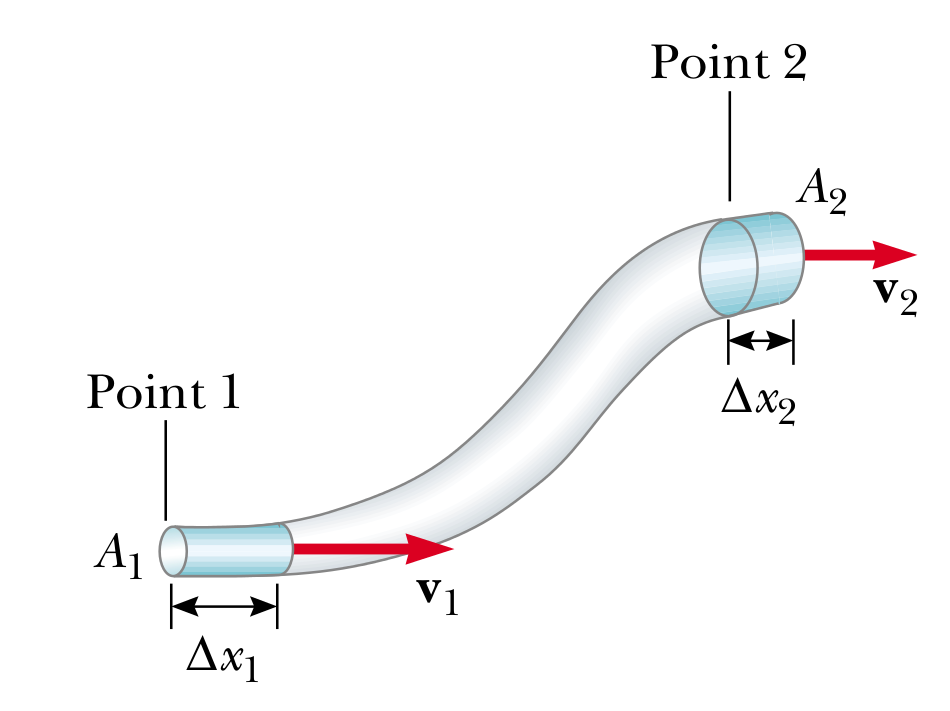
\includegraphics[width=0.45\textwidth]{images/tuboS}
\end{center}
\end{frame}

\begin{frame}
    \begin{itemize}
        \item A quantidade $I_M=\rho A v$ é chamada de \textbf{vazão mássica}
        \item As dimensões de $I_M$ são as de massa dividida por tempo
        \item A massa que atravessa a superfície 2 durante o mesmo tempo $\Delta t$ é:
    \end{itemize}
\[
\Delta m_2 = \rho_2 A_2 v_2 \Delta t
\]
\begin{center}
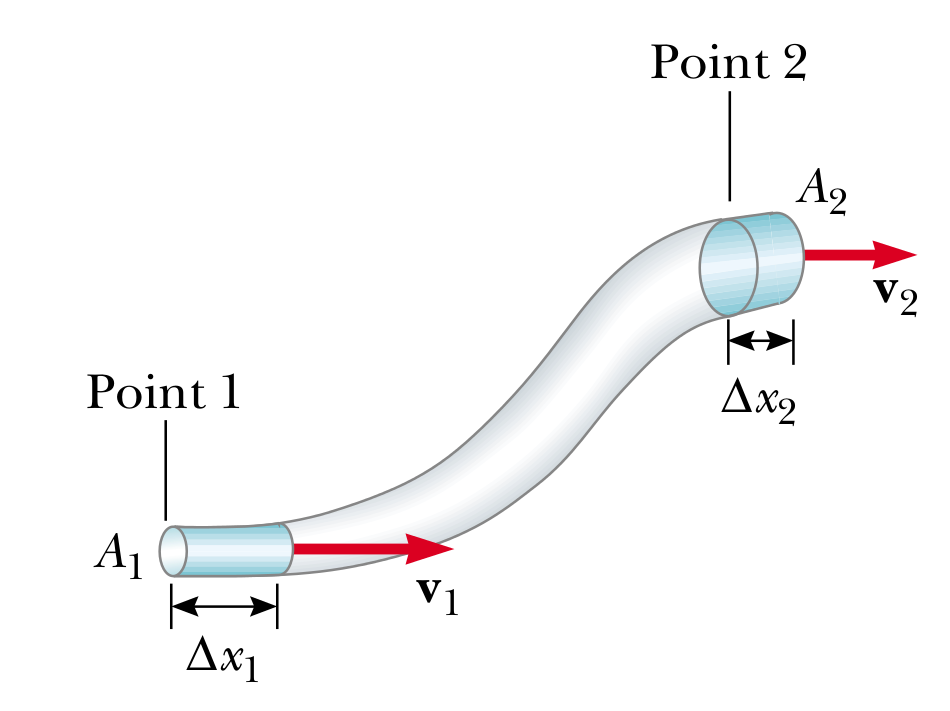
\includegraphics[width=0.45\textwidth]{images/tuboS}
\end{center}
\end{frame}

\begin{frame}[c]
A diferença entre a taxa na qual massa entra no tubo e a taxa na qual a massa
sai do tubo é igual a taxa de variação da massa do tubo:
\[
\frac{\Delta m_1}{\Delta t} - \frac{\Delta m_2}{\Delta t} = \frac{dm}{dt} ~\rightarrow~ I_{M1}-I_{M2} = \frac{dm}{dt}
\]
essa equação é chamada de \textbf{equação da continuidade}.
\end{frame}

\begin{frame}
Escoamento no qual o movimento do fluido é constante (não varia com o tempo) em
todos os pontos é chamado \textbf{estacionário}. Em um escoamento estacionário
a vazão mássica em um dado instante é a mesma através de todas as superfícies
de seção reta.Além disso, a vazão mássica é constante.

\[
\frac{dm}{dt}=0 ~\rightarrow~ I_{M1}=I_{M2}
\]

A quantidade $I_V = Av$ é chamada de \textbf{vazão volumétrica}. Para um fluido incompressível, temos:
\[
I_{V1}=I_{V2}
\]
\end{frame}

\begin{frame}{Exemplo}
A figura abaixo mostra dois segmentos de uma antiga tubulação que atravessa uma
colina: as dimensões são \(d_A = \SI{30}{m}\), \(d_B=\SI{35}{m}\) e
\(D=\SI{115}{m}\). O raio do cano do lado de fora da colina é \SI{2.00}{cm}; o
raio do cano no interior da colina, porém, não é mais conhecido. Para
determiná-lo, os engenheiros hidráulicos verificaram inicialmente que a
velocidade da água nos segmentos à esquerda e à direita da colina era
\SI{2.50}{m/s}. Em seguida, introduziram um corante na água no ponto \(A\) e
observaram que levava \SI{100}{s} para chegar ao ponto \(B\). Qual é o raio
médio do cano no interior da colina?

\begin{center}
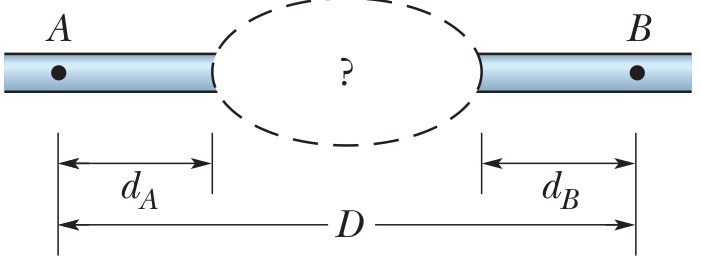
\includegraphics[width=0.4\textwidth]{images/colina}
\end{center}

\end{frame}

\begin{frame}{Equação de Bernoulli}
A equação de Bernoulli relaciona a pressão, a altura e a velocidade (módulo) de
um fluido \textbf{incompressível não-viscoso em escoamento estacionário}:
\[
P_2+\rho g h_2 + \frac{1}{2}\rho v^2_2 = P_1+\rho g h_1 + \frac{1}{2}\rho v^2_1
\]

A equação de Bernoulli pode ser enunciada, também, como
\[
P+\rho g h + \frac{1}{2}\rho v^2 = \mathrm{constante}
\]

Para um fluido em repouso, temos:
\[
P+\rho g h = \mathrm{constante}
\]
\end{frame}

\begin{frame}{Exemplos não copiados}
    Resolva os problemas 57, 58, 69, 71 e 83 do capítulo 14 do livro texto
\end{frame}

\begin{frame}{Exemplos rabiscados}
\begin{itemize}
    \item Problema 70
    \item Problema 71
\end{itemize}
\end{frame}

% \begin{frame}{Exemplo - Lei de Torricelli}
% Um grande tanque de água, aberto em cima, possui um pequeno furo lateral a uma
% distância $\Delta h$ abaixo da superfície da água. Determine a velocidade com
% que a água sai do furo.
% \end{frame}

% \begin{frame}{Medidor Venturi}

% Um \textit{medidor Venturi} é mostrado na figura abaixo. Expresse a velocidade
% \(v_1\) em termos da altura medida \(\Delta h\) e das grandezas conhecidas
% \(\rho_F\), \(\rho_L\) e \(r=A_1/A_2\)

% \begin{center}
% 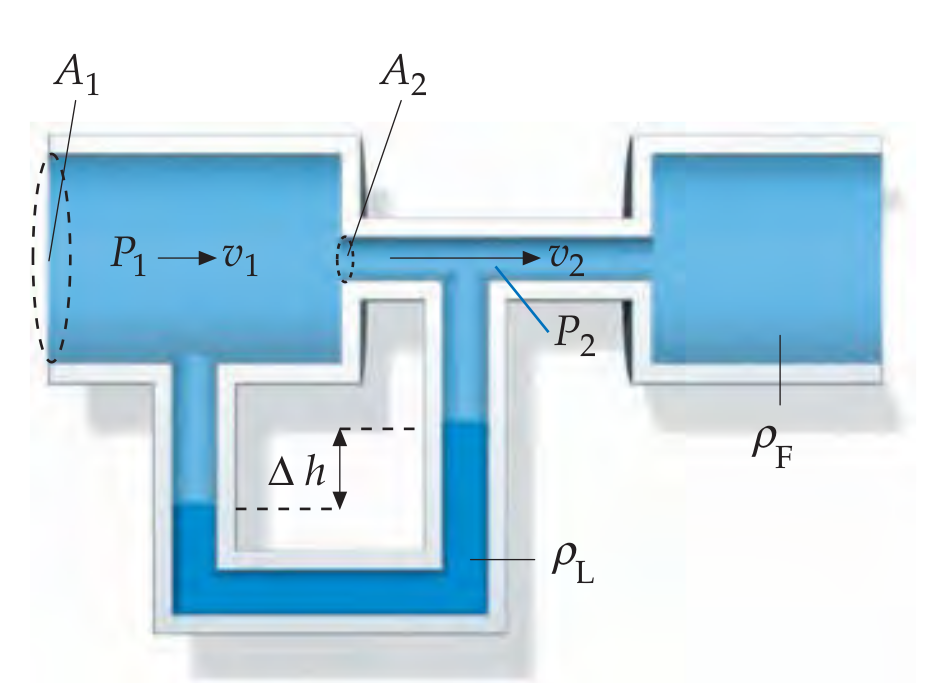
\includegraphics[width=0.5\textwidth]{images/venturi}
% \end{center}
% \end{frame}
